\documentclass{report}

\usepackage{a4}
\usepackage[hypertex]{hyperref}
\usepackage{graphicx}


\begin{document}

\title{Exploring Machine Learning:\\
  The ID3 algorithm}

\author{Mohammed Ibrahim\\
 Computer Science Department\\
  College of Science, Swansea University\\
  Swansea, SA2 8PP, UK
}

\maketitle

\tableofcontents

\chapter{File Format}
\label{sec:fileformat}

\section{File Format}
\label{sec:file}

A file format is a specific way that information is encoded for storage in a computer file. There are different kinds of file formats for different kinds of information. Some file formats are designed for very particular sorts of data.
Syntax: The form or structure of the expressions, statements, and program units. Semantic: The meaning of the expressions, statement, and program units. ???	

line 1: comments ???\\
attribute(1), attribute(2), attribute(3), attribute(n); ???


\begin{enumerate}
\item Comments are ignored in the file. ??? how do we recognise a comment? ???
\item The first line is a comment ??? false ??? , hash symbol signifies ??? a comment and the program reads the first line and ignores it. 
\item The program only accept upper-case (A-Z) ,lower-case (a-z) and digits (0-9). These are the letters we allowed  in a file. ??? this is false ???
\item The second line will reads the number of attribute from the given training set. ??? false ???
\item The program splits the attributes explicitly in second line by using commas and space to separate each attributes in training set. The example attributes are given below. ??? no commas ???
\item The program will read the first column $<Day>$ attribute from the training set with their possible values. ??? Day ???
\item The program will read the second column$<Outlook>$ attribute from the training set with their possible values.
\item The program will read the third column $<Temperature>$ attribute from the training set with their possible values.
\item The program will read the fourth column $<Humidity>$ attribute from the training set with their possible values.
\item The program will read the fifth column $<Wind>$ attribute from the training set with their possible values. 
\item The program will read the Target attribute $<Play>$ from the training set with their possible values.

\end{enumerate}

{\bf Restrictions}

\begin{itemize}

\item The first line of a program has to be ignored as comment.
\item The first column is defined as an Integer and others are Strings.
\item The number of possible values should be same as the number of attributes.
\item The values in the last column should only be ``yes' or ``no'.
\item The first column should be x1={sunny,overcast,rain}.
\item The second column should be x2 ={hot, mild, cool}.
\item The third column should be x3 ={high, normal}
\item The fourth column should be x4={weak, strong}
\item The last column (target attribute) should be x5={yes, no}\\\\


{\bf Example format:}\\
Example from [Mitchell, Machine Learning], Chapter 3, Page 59\\
The above line is a commented line, the program ignores the line.

Day, outlook, temperature, humidity, wind, play
The above line is the second line in the program, where the attributes are separated using comma's and space. 
 
1, sunny, hot, high, weak, no\\
2, sunny, hot, high, strong, no\\

The above values use the space and comma's to separate the data. Here each component of the string is used to separate the data.


\end{itemize}


\subsection{End-Of-Line}
\label{sec:Eol}

Every file has End-of-line(EOL) symbol and file terminates with the end of line symbol, the end-of-line symbols are invisible.
There are three possibilities including end-of-line symbol in the file.
\begin{enumerate}

\item The programs declares syntax error not having end-of-line symbol.
\item The programs doesn't show any error, it just accept it.
\item The programs displays a warning message stating that there is no end-of-line symbol.

\end{enumerate}

There are 3 line end conventions in common use: CR (MacOS), LF (Unix) and CRLF (Windows). CR 
and LF here refer to characters with ASCII code 13 and 10 respectively. 
Different operating systems use different character sequence to indicate the end-of-line in a text file.
Every single line has end-of-line symbol and it takes 1 byte.




\section{Comma-separated values}
\label{sec:csv}

To refer from \cite{Wikipedia_CommaSeparatedValues}(page 1): A comma-separated values(CSV) file stores tabular data(numbers and text)in plain text form. Plain text means that the file is a sequence of characters, with no data that has to be interpreted instead, as binary numbers. A CSV file consists of any number of records, separated by line breaks of some kind; each record consists of fields, separated by some other character or string, most commonly a literal TAB or comma. Usually, all records have an identical sequence of fields.


\section{Identifiers}
\label{sec:ide}

According to \cite{Roberts2000CompleteJava2Certification}(Chapter 1, page 6): An identifier is a name used by a programmer to variable, method, package, class, interfaces or label. Keywords and reserved words can't be used as  identifiers. It must begin with a letter, a dollar sign, or an underscore; identifiers are case sensitive. Identifiers are tokens (also called symbols) which name as language entities. Each variable has a name by which it is identified in the program.

\section{Decision Tree}
According to \cite{Mitchell1997MachineLearning}(page 59,Chapter 3): Training set : In machine learning training sets are generally called as tables, where each row in the table represents a single training example. 

To illustrate the operation of ID3, we consider the learning task represented by the example training set given in Figure \ref{fig:trainingplaytennis}. We have four attributes Outlook, Temperature, Humidity and Wind. The target attribute is called PlayTennis, which has values boolean value \texttt{yes} or \texttt{no} for different Saturday mornings, is to be predicted based on other attributes of the morning in question.
\begin{figure}[h]
  \centering
  \begin{tabular}{|c|l|l|l|l|l|l|}
    \hline
    Day & Outlook & Temperature & Humidity & Wind & PlayTennis\\
    \hline
    1 & sunny & hot & high & weak & no
    \\\hline
    2 & sunny & hot & high & strong & no
    \\\hline
    3 & overcast & hot & high & weak & yes
    \\\hline
    4 & rain & mild & high & weak & yes
    \\\hline
    5 & rain & cool & normal & weak & yes
    \\\hline
    6 & rain & cool & normal & strong & no
    \\\hline
    7 & overcast & cool & normal & strong & yes
    \\\hline
    8 & sunny & mild & high & weak & no
    \\\hline
    9 & sunny & cool & normal & weak & yes
    \\\hline
    10 & rain & mild & normal & weak & yes
    \\\hline
    11 & sunny & mild & normal & strong & yes
    \\\hline
    12 & overcast & mild & high & strong & yes
    \\\hline
    13 & overcast & hot & normal & weak & yes
    \\\hline
    14 & rain & mild & high & strong & no
    \\\hline
  \end{tabular}
  \caption{Training set for \texttt{PlayTennis} example}
  \label{fig:trainingplaytennis}
\end{figure}

\begin{figure}[h]
\centering
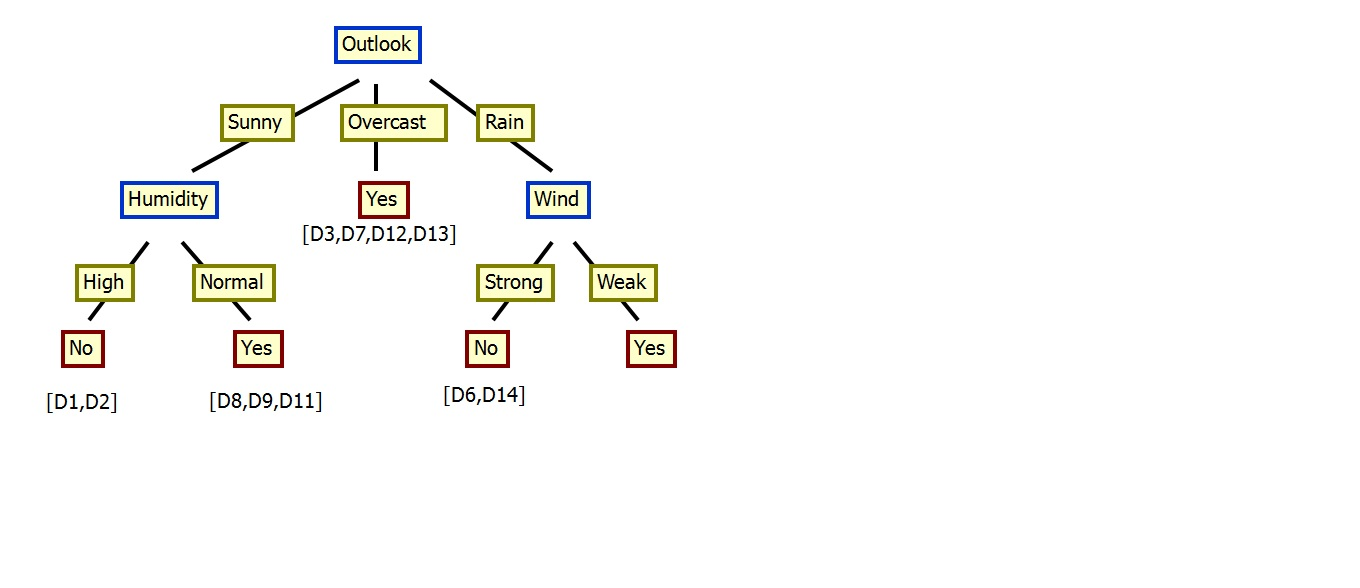
\includegraphics[bb=0 0 1360 588,scale=0.5,keepaspectratio=true]{DecisionTree.jpg}
\caption{Decision Tree}
\label{fig:decisiontree}
\end{figure}
The below figure shows the complete decision tree for the above training set.\ref{fig:decisiontree}\\


{\bf The decision tree can be expressed in rule format:}\\	

IF outlook = sunny AND humidity = high THEN playball = no

IF outlook = rain AND humidity = high THEN playball = no

IF outlook = rain AND wind = strong THEN playball = yes

IF outlook = overcast THEN playball = yes

IF outlook = rain AND wind = weak THEN playball = yes\\

The below decision tree shows the concept for PlayTennis. An example is classified by sorting it through the tree to appropriate leaf node,then returning the classification associated with this leaf ( Yes or No ). The below tree classifies the Saturday mornings according to whether or not they are suitable for playing tennis.

\begin{itemize}

\item The idea of decision tree is sorting them down the tree from the root to leaf node, which will provide the classification of instance.
\item Each node in the decision tree states the some attribute of the instance.
\item Each branch descending from that node corresponds to one of the possible values of this attribute.
\item An instance is classified by starting at the root node of the tree,testing the attribute specified by this node, then moving down the tree branch corresponding to the value of the attribute in the given example.
\item This process is repeated for the sub tree rooted at the new node

\end{itemize}

The decision tree is constructed using the techniques of ID3 algorithm. The following steps should follow to construct the decision tree.

According to the book of \cite{Mitchell1997MachineLearning} (page 56, chapter 3) ID3(Examples, target-attribute, attribute)
\begin{itemize}
\item Examples : are the training examples \ref{fig:trainingplaytennis}
\item target-attribute : is the attribute whose value is to be predicted by the tree.
\item Attributes : is a list of other attributes that may be tested by the learned decision tree.\\
Returns a decision tree that correctly classifies the given examples.\\
\end{itemize}


\begin{tabbing}
Create a root node for the tree\\
If \= all examples are positive, Return the single-node tree Root, with label = +.\\
If \= all examples are negative, Return the single-node tree Root, with label = -.\\
If \= Attributes is empty, Return the single-node tree Root, with label = most common value of\\ target attribute in Examples\\
Otherwise Begin \\
\> then \=  A = The Attribute that best classifies examples.\\
\> Decision Tree attribute for Root = A.\\
\> For each possible value, vi, of A,\\
\> \> Add a new tree branch below Root, corresponding to the test A = vi.\\
\> \> Let Examples(vi) be the subset of examples that have the value vi for A\\
\> \> If Examples(vi) is empty\\
\> \> Then below this new branch add a leaf node with label = most\\
\> \> common target value in the examples\\
\> \> Else below this new branch add the subtree ID3 \\
\> \> (Examples(vi), target attribute, Attributes – {A})\\

end\\
return Root\\
\end{tabbing}

Training set : \cite{RuleInduction}(Page 1):

\begin{figure}[h]
  \centering
  \begin{tabular}{|c|l|l|l|l|l|l|}
    \hline
   Slno & Skin	& Colour & Size & Flesh & Conclusion\\
    \hline
    1 & hairy &	brown &	large &	hard & safe	
    \\\hline
    2 & hairy & green & large & hard & safe
    \\\hline
    3 & smooth & red & large & soft & dangerous
    \\\hline
    4 & hairy & green & large & soft & safe	
    \\\hline
    5 & hairy &	red & small	& hard	& safe
    \\\hline
    6 & smooth & red & small & hard & safe	
    \\\hline
    7 & smooth & brown & small & hard &	safe	
    \\\hline
    8 & hairy &	green &	small &	soft & dangerous	
    \\\hline
    9 & smooth & green & small & hard &	dangerous
    \\\hline
    10 & hairy & red & large & hard & safe
    \\\hline
    11 & smooth & brown & large & soft & safe	
    \\\hline
    12 & smooth	& green & small	& soft	& dangerous
    \\\hline
    13 & hairy	& red & small & soft & safe	
    \\\hline
    14 & smooth	& red &	large &	hard & dangerous
    \\\hline
    15 & smooth & red & small &	hard & safe
    \\\hline
    16 & hairy & green & small & hard & dangerous		
    \\\hline
                 
    
  \end{tabular}
  \caption{Training set for \texttt{FoodExample} example}
  \label{fig:foodexample}
\end{figure}



\begin{figure}[h]
  \centering
  \begin{tabular}{|c|l|l|l|l|l|l|}
    \hline
    AGE & COMPETITION & TYPE & PROFIT\\
    \hline
    old	& yes & software & down
    \\\hline
    old & no & software & down
    \\\hline
    old	& no & hardware & down
    \\\hline
   	mid	& yes & software & down
    \\\hline
    mid	& yes & hardware & down
    \\\hline
    mid & no & hardware & up
    \\\hline
    mid & no & software & up
    \\\hline
    new & yes & software & up
    \\\hline
    new & no & hardware	& up
	\\\hline
	new	& no & software	& up
	\\\hline
   
  \end{tabular}
  \caption{Training set for \texttt{StockExample} example}
  \label{fig:stockexample}
\end{figure}





\bibliographystyle{plain}
\bibliography{Bibliography}



\end{document}